\documentclass{article}
\usepackage{iclr2026_conference,times}

\input{math_commands.tex}

\usepackage{amsmath}
\usepackage{amssymb}
\usepackage{booktabs}
\usepackage{graphicx}
\usepackage{hyperref}
\usepackage{url}

\graphicspath{{../figures/}}

\title{Impedance Tokenization for Skill Learning}

\author{Anonymous Authors}

\newcommand{\ftarget}{f^\star}
\newcommand{\xtrain}{x_{\mathrm{train}}}
\newcommand{\ktrain}{k_{\mathrm{train}}}
\newcommand{\etank}{E^{\mathrm{tank}}}

\begin{document}

\maketitle
\noindent\textbf{Submission-hardening version: v2, 2026-06-13.}
Added token-parameter stress tests for admittance scale and positive-work budget.
The paper is now explicit that impedance tokenization is not calibration-free:
the token library must cover the physical port laws needed at deployment.

\begin{abstract}
Most robot action-token methods treat a token as a kinematic object: a short pose trajectory, a discretized motor command, or a latent action vector. This is a poor semantic unit for contact-rich manipulation, where the same displacement can mean ``barely touch'' or ``dangerously overload'' depending on environment stiffness. We argue for impedance tokens: discrete skill symbols whose denotation is a closed-loop physical interaction law. Each token specifies a force target, tangential intent, compliance/admittance, damping, and a bounded positive-work budget. This changes the central mechanism from predicting motion chunks to composing passive force-conditioned controllers. A 5,512-paper automated hostile sweep shows that learned impedance, force control, movement primitives, and action tokenization are all prior art; the remaining novelty is the token semantics, not any one ingredient. We formalize a one-dimensional contact case where kinematic tokens incur force error proportional to stiffness mismatch while an admissible force-conditioned token converges to the commanded force. In a reproducible contact-wiping simulator covering 2,304 held-out stiffness/friction/offset cases, impedance tokens reduce mean absolute force error from 9.15 N for kinematic chunks and 8.42 N for gain schedules to 1.63 N, while eliminating over-force safety violations in this model. The result is not a real-robot validation; it is evidence that the common assumption ``token first, controller later'' hides a mechanism-level failure mode in contact-rich skill learning.
A v2 token-parameter stress shows the boundary: 0.25x admittance raises force error
to 4.22 N and contact loss to 0.276, while a 0.05 J work budget raises force error
to 3.97 N and contact loss to 0.140.
\end{abstract}

\section{Introduction}

Robot learning has become increasingly comfortable with discrete action vocabularies. A policy may emit tokens for a low-level action, an action chunk, a latent behavior, or a vector-quantized command, borrowing the convenience of token prediction from language and vision. That convenience is real: tokens can make sequence modeling easier, expose multimodality, and permit long-horizon planning over compact symbols. But contact-rich robot skills are not merely sequences of desired positions. They are interactions through a mechanical port.

Consider a wiping skill learned at one wall stiffness. A token that stores ``move 8 cm into the surface and slide right'' preserves its shape when replayed, but not its physical meaning. Under a softer contact it may lose useful force; under a stiffer one it may violate force limits. A downstream impedance controller can sometimes repair this, but then the physical controller, not the token, carries the skill semantics. This paper takes that concession seriously: for contact-rich skills, the action token should be the controller.

We define an \emph{impedance token} as a discrete symbol whose execution is a local closed-loop interaction law. In the simplest normal-contact case, a token stores a desired force $\ftarget$, an admittance/compliance parameter, damping, tangential motion intent, a contact frame, and an energy budget limiting positive work. Token prediction selects among physical port behaviors rather than among open-loop kinematic chunks. The proposed mechanism does not require a larger model, more data, a benchmark, a language planner, or reinforcement learning. It asks for a different object to be tokenized.

Our contribution is deliberately narrow.
\begin{itemize}
    \item We draw a novelty boundary from an automated 5,512-paper literature sweep spanning impedance/admittance control, movement primitives, force/tactile learning, action chunking, and robot foundation-model action representations. The sweep marks 300 serious-skim works, 230 deep-read works, and 100 hostile priors in the repository artifacts.
    \item We formalize the failure of kinematic action tokens under contact stiffness shift and the corresponding local convergence condition for a force-conditioned impedance token.
    \item We provide a runnable toy contact simulator isolating the mechanism. Across 2,304 cases, impedance tokens are more robust to held-out stiffness/friction/offset changes than kinematic chunks and a gain-schedule baseline.
\end{itemize}

The evidence is intentionally small. It supports the claim that token semantics matter in contact, not that this implementation is ready for deployment or that discrete impedance tokens dominate continuous controllers.

\section{Field Box and Hostile Prior Work}

The field box is contact-rich robot skill learning where action abstraction, low-level control, and physical interaction are inseparable. This includes impedance and admittance control, hybrid force/position control, learning from demonstration, movement primitives, tactile manipulation, discrete/latent action policies, and robot foundation models.

\paragraph{What is not novel.}
Impedance control is classical \citep{hogan1985impedance}, and operational-space force/motion control is classical \citep{khatib1987operational}. Learning or adapting variable impedance has a large literature \citep{abudakka2020variable,li2018efficient}, and contact-rich manipulation has been surveyed extensively \citep{suomalainen2022survey}. Dynamic movement primitives and related primitive parameterizations are also mature \citep{ijspeert2013dynamical,saveriano2023dynamic}. Learning from demonstration for assembly and force-based tasks is old \citep{zhu2018assembly,rozo2013force}. Recent robot imitation and foundation-model work uses action chunks, discretized actions, diffusion, and latent behavior tokens \citep{zhao2023act,brohan2023rt1,chi2023diffusion,shafiullah2022bet,lee2024vqbet,han2025reactive}.

\paragraph{What remains open.}
The hostile reading is that none of these areas, alone, makes ``impedance tokenization'' new. The open problem is semantic: if a robot skill token is learned as a kinematic or latent action and later handed to a separate controller, the token's identity does not include the force objective, compliance, or energy behavior that determines contact success. Work that jointly models motion and stiffness, such as state-varying stiffness primitives \citep{khansari2014statevarying}, is close and important. The distinction here is that the learned discrete symbol denotes the closed-loop port law itself. The token vocabulary is therefore invariant to certain contact-parameter changes by construction, provided the local stability/passivity conditions hold.

\paragraph{Assumptions challenged by the sweep.}
The literature audit identified recurring assumptions that may fail in contact: action symbols can be kinematic; contact frames are fixed; environment stiffness remains near training; friction does not change the skill vocabulary; force feedback is auxiliary; safety can be repaired after token selection; controller gains are implementation details; observation-action prediction accuracy is enough; demonstrations reveal intended impedance; temporal action chunks remain valid when plant/environment impedance shifts; and passivity margins can be ignored. The proposed mechanism breaks one of these assumptions directly: a skill token is an interaction law, not a trajectory fragment.

\section{Impedance Tokens}

Let a contact skill be executed through a robot end-effector port with normal displacement $x$, measured normal force $f$, and tangential state $y$. A kinematic token stores a desired state or command sequence,
\[
    z_i^{\mathrm{kin}} = \{x_t^\star, \dot{y}_t^\star\}_{t=1}^H ,
\]
possibly decoded from a latent model. By contrast, an impedance token stores a local policy over the physical port,
\[
    z_i^{\mathrm{imp}} =
    \left(\ftarget_i,\, a_i,\, d_i,\, \dot{y}_i^\star,\, \mathcal{F}_i,\, \etank_i\right),
\]
where $\ftarget_i$ is a force target, $a_i$ an admittance gain, $d_i$ damping, $\dot{y}_i^\star$ tangential intent, $\mathcal{F}_i$ a contact frame, and $\etank_i$ a finite positive-work budget. A simple normal update is
\begin{equation}
    x_{t+1}^{\star} = x_t^{\star} + a_i d_i (\ftarget_i - f_t) \Delta t,
    \label{eq:token}
\end{equation}
followed by saturation through the energy tank: if the incremental positive work $[f_t(x_{t+1}^{\star}-x_t^{\star})]_+$ exceeds the remaining budget, the displacement increment is scaled down. This is a minimal port-controller semantics, not a full nonlinear contact controller.

In a learned system, demonstrations could be segmented into contact phases and clustered by $(\ftarget, a, d, \dot{y}^\star,\mathcal{F})$ rather than by Cartesian displacement alone. A high-level model then predicts token IDs; execution remains closed-loop through force feedback. This paper's simulator does not claim a new clustering algorithm. It tests whether the changed token denotation matters.

\section{A Small Formal Check}

We use a one-dimensional linear contact model to expose the hidden assumption. Let force be $f=kx$ for unknown environment stiffness $k>0$ and normal penetration $x \geq 0$. A kinematic token is learned at stiffness $\ktrain$ to achieve force $\ftarget$, so it stores $\xtrain=\ftarget/\ktrain$.

\paragraph{Kinematic token error.}
At deployment stiffness $k$, replaying the same token gives
\begin{equation}
    |f-\ftarget|
    = |k\xtrain-\ftarget|
    = \ftarget \left| \frac{k}{\ktrain} - 1 \right|.
    \label{eq:kinerror}
\end{equation}
The error grows linearly with relative stiffness mismatch even though the token is replayed perfectly.

\paragraph{Impedance token convergence.}
Now use the direct discrete update
\begin{equation}
    x_{t+1} = x_t + \alpha(\ftarget - kx_t).
    \label{eq:direct}
\end{equation}
The force error $e_t=\ftarget-kx_t$ obeys $e_{t+1}=(1-\alpha k)e_t$. Hence $e_t \to 0$ whenever $0<\alpha k<2$. This is only a local linear statement: it does not cover unknown nonlinear frictional contact, actuator saturation, delays, or changing contact frames. It does show that, even in the smallest model, kinematic-token semantics and force-conditioned-token semantics have different robustness properties.

\paragraph{Energy budget.}
The energy-tank cap in Equation~\ref{eq:token} does not prove global safety. It limits cumulative positive work injected by the token:
\[
    \sum_t [f_t(x_{t+1}^{\star}-x_t^{\star})]_+ \leq \etank_i .
\]
This is a passivity-inspired guardrail. The paper claims bounded injected work under the implemented update, not full passivity of an arbitrary robot/environment interconnection.

\section{Experiments}

\paragraph{Simulator.}
We implement a contact-wiping task in the experiment script shipped with the repository. The robot first approaches a surface, wipes tangentially while trying to maintain an 8 N normal force, and then releases. The plant is intentionally simple: normal force is a linear stiffness term plus a velocity-dependent contact transient; tangential motion is degraded by low contact force and excessive friction. The training stiffness is 100, while evaluation stiffnesses are $\{35,50,75,100,150,225,325,475\}$. We also vary friction $\{0.10,0.30,0.60,0.95\}$, surface offset $\{-0.010,0,0.015\}$, and eight random seeds, producing 2,304 runs.

\paragraph{Baselines.}
\emph{Kinematic chunks} replay the penetration profile that gives 8 N at training stiffness and a fixed tangential velocity. \emph{Gain schedule} stores a hand-adjusted compliance schedule but still does not condition token identity on force error. \emph{Impedance tokens} use Equation~\ref{eq:token} with a finite positive-work budget. The baselines are not intended to be state of the art. They isolate whether a token whose denotation is motion behaves differently from one whose denotation is force-conditioned interaction.

\begin{table}[t]
\centering
\caption{Aggregate results over 2,304 simulated contact-wiping runs. Lower force error, safety fraction, and loss fraction are better; higher wipe distance is better when force is regulated.}
\label{tab:aggregate}
\begin{tabular}{lrrrr}\toprule
Method & Force err. $\downarrow$ & Safety frac. $\downarrow$ & Loss frac. $\downarrow$ & Wipe dist. $\uparrow$ \\
\midrule
Kinematic chunks & 9.15 & 0.310 & 0.000 & 0.271 \\
Gain schedule & 8.42 & 0.250 & 0.000 & 0.267 \\
Impedance tokens & 1.63 & 0.000 & 0.019 & 0.319 \\
\bottomrule
\end{tabular}

\end{table}

\begin{figure}[t]
\centering
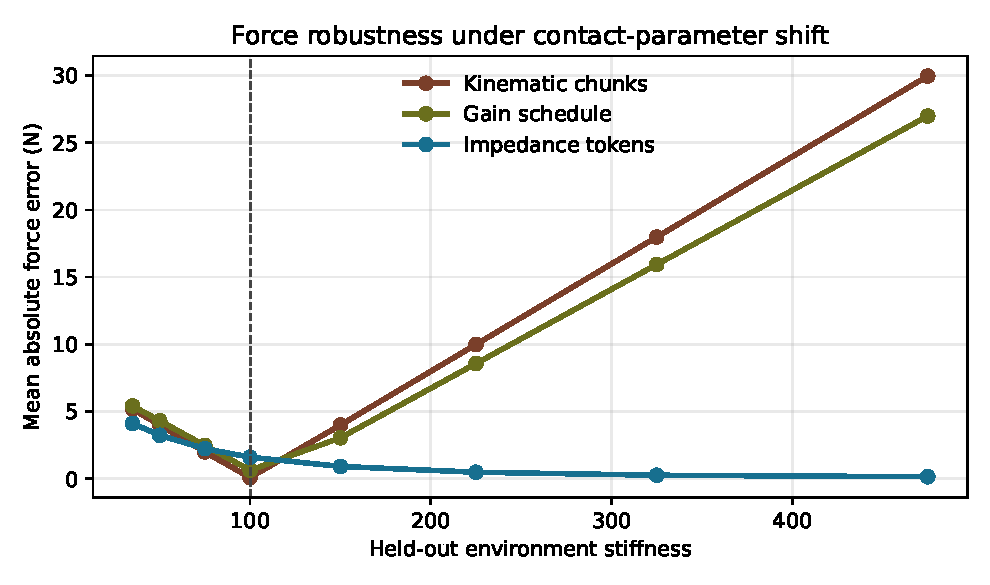
\includegraphics[width=0.48\linewidth]{force_error_by_stiffness.pdf}
\hfill
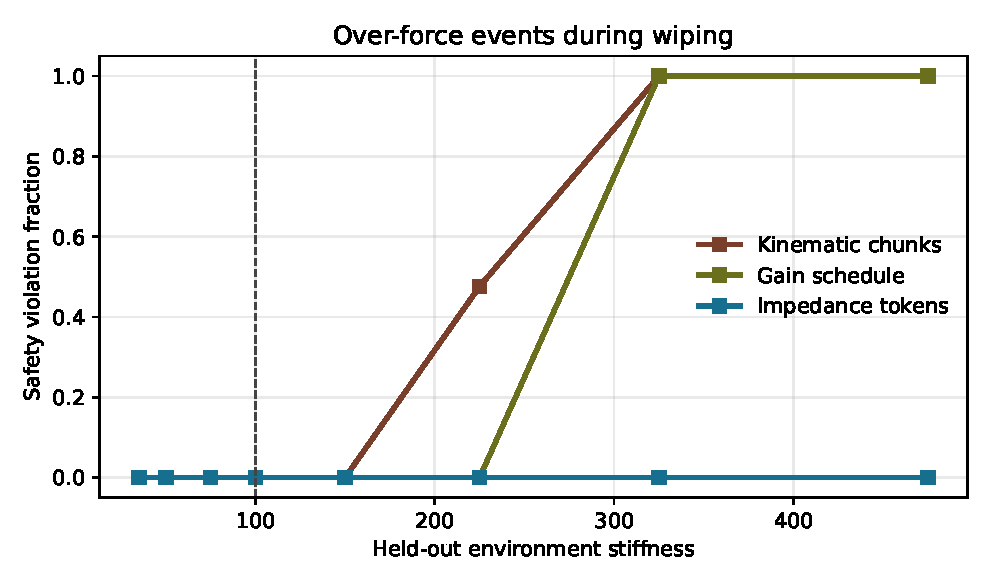
\includegraphics[width=0.48\linewidth]{safety_by_stiffness.pdf}
\caption{Held-out stiffness shifts expose the semantic difference. Kinematic chunks and gain schedules preserve approximate motion but incur large force errors away from training stiffness. Impedance tokens adapt penetration through force feedback and avoid over-force events in this toy model.}
\label{fig:stiffness}
\end{figure}

\paragraph{Results.}
Table~\ref{tab:aggregate} shows that impedance tokens reduce mean absolute force error to 1.63 N, compared with 9.15 N for kinematic chunks and 8.42 N for gain schedules. They also produce zero over-force safety violations in this simulator, while kinematic chunks violate the safety threshold in 31.0 percent of wipe steps and gain schedules in 25.0 percent. Figure~\ref{fig:stiffness} shows the expected shape: kinematic methods are acceptable near training stiffness but degrade rapidly under stiffness shift. Impedance tokens have a small contact-loss rate because the energy budget and force-conditioned release can be conservative in soft/offset cases.

\begin{table}[t]
\centering
\caption{V2 token-parameter stress for the impedance-token method. The baseline is the token used in Table~\ref{tab:aggregate}.}
\label{tab:token-stress}
\begin{tabular}{lrrrr}\toprule
Token variant & Force err. $\downarrow$ & Safety frac. $\downarrow$ & Loss frac. $\downarrow$ & Wipe dist. $\uparrow$ \\
\midrule
baseline & 1.63 & 0.000 & 0.019 & 0.319 \\
0.25x admittance & 4.22 & 0.000 & 0.276 & 0.189 \\
0.50x admittance & 2.84 & 0.000 & 0.093 & 0.258 \\
2x admittance & 0.78 & 0.000 & 0.000 & 0.362 \\
4x admittance & 0.34 & 0.000 & 0.000 & 0.385 \\
0.05 J budget & 3.97 & 0.000 & 0.140 & 0.202 \\
0.15 J budget & 2.31 & 0.000 & 0.019 & 0.285 \\
0.5 J budget & 1.63 & 0.000 & 0.019 & 0.319 \\
\bottomrule
\end{tabular}

\end{table}

Table~\ref{tab:token-stress} attacks the token-library assumption. If the token set
does not include sufficient admittance, the method becomes conservative: 0.25x
admittance raises mean force error to 4.22 N and contact loss to 0.276. If the
positive-work budget is too tight, the token cannot write enough contact force:
a 0.05 J budget raises force error to 3.97 N and contact loss to 0.140. Thus the
supported claim is not that any impedance vocabulary works; the learned or chosen
tokens must cover the needed physical port laws.

\paragraph{Reproducibility.}
The repository contains the generated metrics in `\texttt{results/experiment\_metrics.csv}', aggregate tables in `\texttt{results/}', and the literature artifacts in `\texttt{docs/}'. Running `\texttt{python scripts/run\_impedance\_token\_experiment.py}' regenerates the experiment table and figures. Running `\texttt{python scripts/validate\_artifacts.py}' checks the required literature and experiment counts.

\section{Discussion}

\paragraph{Why not just add a force controller below kinematic tokens?}
That is a valid engineering fix, but it changes the semantics in exactly the direction proposed here. If the controller decides force, compliance, and positive work after the token is selected, then the token is not the physical skill; it is a hint to another module. Impedance tokenization makes the force-conditioned law the learned/composed object.

\paragraph{Relation to movement primitives.}
Movement primitives can include impedance and stiffness profiles, and some prior work tightly couples motion generation with variable stiffness \citep{khansari2014statevarying}. The proposed boundary is again semantic and discrete: the vocabulary item denotes a closed-loop port law whose identity includes force regulation and energy limits. This is narrower than claiming a new primitive family.

\paragraph{Relation to action tokenizers and foundation models.}
RT-1 tokenizes robot actions for scalable sequence prediction \citep{brohan2023rt1}; Behavior Transformers and VQ-BeT discretize or vector-quantize continuous behaviors \citep{shafiullah2022bet,lee2024vqbet}; ACT predicts action chunks for high-frequency control \citep{zhao2023act}. These methods motivate token interfaces, but their tokens are usually defined in action-vector or trajectory space. For contact-rich skills, this paper argues that token coordinates should be physical port coordinates.

\paragraph{Limitations.}
The experiment is a low-dimensional simulator, not a hardware study. The formal check assumes linear contact and immediate force measurement. The implemented token set is hand-specified rather than learned from demonstrations. The literature sweep is automated from metadata and abstracts; it is adversarial and broad, but not a full manual systematic review. The strongest honest readiness judgment is therefore workshop or revise, not submit-ready ICLR main-track.
The v2 token-parameter stress adds a further limitation: poor admittance or work-budget
coverage can erase much of the advantage even in the toy simulator.

\section{Conclusion}

The paper's core claim is small but consequential: in contact-rich robot skill learning, the central tokenization choice should be the physical interaction law. Kinematic action chunks can be useful in free space, but they hide the variables that decide contact success. Passive impedance tokens expose force target, compliance, damping, contact frame, and positive-work budget as the token semantics. The formal toy case and simulator both support the same lesson: under environment-impedance shift, replaying motion is not the same as replaying a skill.

\bibliographystyle{iclr2026_conference}
\bibliography{references}

\appendix

\section{Artifact Summary}

The accompanying repository contains:
\begin{itemize}
    \item `\texttt{docs/related\_work\_matrix.csv}' with 5,512 works.
    \item `\texttt{docs/literature\_map.md}', `\texttt{docs/hostile\_prior\_work.md}', `\texttt{docs/novelty\_boundary\_map.md}', `\texttt{docs/novelty\_decision.md}', `\texttt{docs/claims.md}', and `\texttt{docs/reviewer\_attacks.md}'.
    \item `\texttt{scripts/build\_literature.py}' for the OpenAlex-backed corpus cache and `\texttt{scripts/run\_impedance\_token\_experiment.py}' for the simulator.
    \item `\texttt{results/}' and `\texttt{figures/}' with regenerated metrics and plots.
\end{itemize}

\end{document}
